% 2017 全国Ⅰ卷 理16：圆形纸片（半径 5）与内接等边三角形 ABC，
% D、E、F 为圆上的点，分别与 BC、CA、AB 构成待折起的等腰三角形
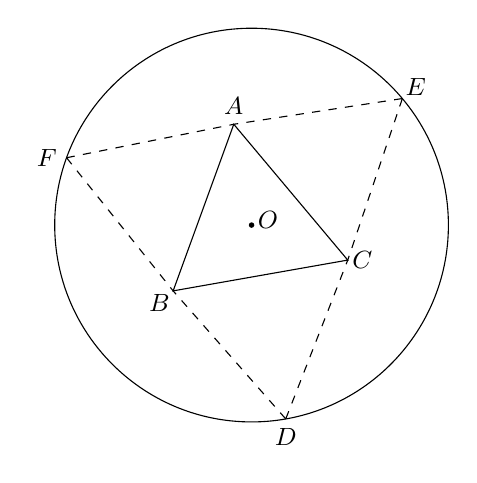
\begin{tikzpicture}[scale=1.0, font=\small]
  \def\R{2.5}      % 圆半径（示意比例）
  \def\r{1.3}      % 三角形中心到顶点距离
  \draw (0,0) circle (\R);
  \coordinate (A) at (100:\r);
  \coordinate (B) at (220:\r);
  \coordinate (C) at (-20:\r);
  \coordinate (D) at (280:\R);
  \coordinate (E) at (40:\R);
  \coordinate (F) at (160:\R);
  \draw (A) -- (B) -- (C) -- cycle;
  \draw[dashed] (D) -- (B) (D) -- (C);
  \draw[dashed] (E) -- (C) (E) -- (A);
  \draw[dashed] (F) -- (A) (F) -- (B);
  \fill (0,0) circle (1pt);
  \node[right, inner sep=1.5pt] at (0.02,0.06) {$O$};
  \node[above] at (A) {$A$};
  \node[below left, inner sep=1pt] at (B) {$B$};
  \node[right, inner sep=1.5pt] at (C) {$C$};
  \node[below] at (D) {$D$};
  \node[above right, inner sep=1pt] at (E) {$E$};
  \node[left] at (F) {$F$};
\end{tikzpicture}
